\documentclass[a4j]{jarticle}
\usepackage{graphicx}
\usepackage{float}
\usepackage{amsmath}
\usepackage{url}

\graphicspath{{./assets/}}
\title{様々なソートアルゴリズム}
\author{クリスティアン ハルジュノ\thanks{釧路工業高等専門学校情報工学科5年情報21番}}
\date{\today}

\begin{document}
\maketitle 
\textbf{事前に} この実験に使用するプログラム, データ, スクリプト等はGitHubの上にホストされています. プログラムを試したり検査したい場合は, 次のURLを参照してください. \\
\begin{center}
  \url{https://tianharjuno.com/sort}
\end{center}
\section{背景}
情報工学における重要な概念の一つにソートアルゴリズムがあります. ソートアルゴリズムの主な目的は, データの配列を最小から最大, または最大から最小の順に並べることです. 一般に, ソートはそれほど複雑な問題ではないと考えられます. しかし, データ量が大幅に増加すると(ビッグデータ企業等), ソートは極めて困難になる場合があります. ソートにかかる時間や使用メモリ量は重要な課題であり, データの種類や量に応じて適切なアルゴリズムを選択する必要があります. また, あるアルゴリズムは効率的ですが, すべてのユースケースに実装する価値がない場合があります. さらに, 多くの会社に応募するとき(Amazon, Google, Netflix, 等), これらの大企業のほとんどは, 実技試験でさまざまな複雑なソートアルゴリズムを実装することを要求しています.\\
\section{一般的のソートアルゴリズム}
この章では, いくつかの有名なソートアルゴリズムについて説明します. これらのアルゴリズムの実装は比較的簡単であり, 効率も高いため, データの種類や量に応じて適切に選択することができます. \\
\subsection{バブルソート}
バブルソートは最もよく知られているソートアルゴリズムの一つです. 実装が非常に簡単であり, 少量のデータに対してはメモリ使用量が少なく, 処理も比較的高速です. この方法にはデータを最初から最後まで調べながら, 現在の数値と次の数値を比較することで機能します. 現在の数値が次の数値よりも大きい場合は, 位置を入れ替えます. このプロセスは, データが完全にソートされるまで何度も繰り返されます.\\
\newpage
\textbf{バブルソートのやり方}
\begin{enumerate}
  \item リストの最初の位置から始める. 
  \item 現在の数値と次の数値を比較する. 
  \item 現在の数値が次の数値より大きければ, 入れ替える. 
  \item 次の位置に進み, リストの末尾までステップ2〜3を繰り返す. 
  \begin{figure}[H]
    \centering
    \includegraphics[width=0.8\linewidth]{bubble1.eps}
    \caption{先頭から末尾まで数値を比較して, 交換する. }
  \end{figure}
  \item 1回の通過が終わったら, 最初の位置に戻って再び通過を行う. 
  \begin{figure}[H]
    \centering
    \includegraphics[width=0.8\linewidth]{bubble2.eps}
    \caption{通過後最初の位置に戻って, 再び通過}
  \end{figure}
  \item 通過中に1回も入れ替えがなければ, ソートは完了. 
  \item 入れ替えがあった場合, ステップ1〜6を繰り返す. 
  \begin{figure}[H]
    \centering
    \includegraphics[width=0.8\linewidth]{bubble3.eps}
    \caption{通過後に入れ替えされた要素がないと終了}
  \end{figure}
\end{enumerate}
バブルソートの計算量はデータの状況によって定義します. \\
\begin{description}
  \item[最良] 最適というのはそのデータを事前にソートされている状態です. 
  \begin{equation}
    \centering
    O(n)
  \end{equation}
  \item[平均] 入力が均一に分布していると仮定して, すべての可能な入力順列に対して実行される操作の予想数です. 
  \begin{equation}
    \centering
    O(n^2)
  \end{equation}
  \item[最悪] 最悪の状態はソート対応するデータが逆順としてソートする状態です. 
  \begin{equation}
    \centering
    O(n^2)
  \end{equation}
\end{description}

\subsection{挿入ソート}
挿入ソートは, 要素を適切な位置に直接挿入することで並べ替えを行うアルゴリズムです.   
現在処理している要素を, それより前の要素と右から左に1つずつ比較し, 比較対象が現在の要素より大きければ, 右にずらします.   
適切な位置が見つかったところで, 現在の要素を挿入します. \\
\textbf{挿入ソートのやり方}
\begin{enumerate}
  \item 最初の要素をソート済み部分とみなす. 
  \item 次の要素を取り出して, ソート済み部分の各要素と比較する. 
  \begin{figure}[H]
    \centering
    \includegraphics[width=0.8\linewidth]{insertion1.eps}
    \caption{第二位置からスタート. ソート済み要素より大きい数値を左にずらす. }
  \end{figure}
  \item ソート済み部分の中で, 自分より大きい要素を右にずらす. 適切な位置に挿入する. 
  \begin{figure}[H]
  \centering
  \includegraphics[width=0.8\linewidth]{insertion3.eps}
    \caption{繰り返して, ソート済み要素より大きい数値を左にずらす}
  \end{figure}
  \item 適切位置がないとそのままで次の位置に進む
  \item リストの末尾までステップ2〜4を繰り返す. 
  \begin{figure}[H]
    \centering
    \includegraphics[width=0.8\linewidth]{insertion2.eps}
    \caption{適切位置がないとそのままで進む}
  \end{figure}
  \item ソートされていない要素がないと終了
  % \begin{figure}[H]
  %   \centering
  %   \includegraphics[width=0.8\linewidth]{insertion4.eps}
  %   \caption{終了}
  % \end{figure}
\end{enumerate}
挿入ソートの計算量はデータの状況によって定義します. 
\begin{description}
  \item[最良] 最適というのはそのデータを事前にソートされている状態です. 
  \begin{equation}
    \centering
    O(n)
  \end{equation}
  \item[平均] 入力が均一に分布していると仮定して, すべての可能な入力順列に対して実行される操作の予想数です. 
  \begin{equation}
    \centering
    O(n^2)
  \end{equation}
  \item[最悪] 最悪の状態はソート対応するデータが逆順としてソートする状態です. 
  \begin{equation}
    \centering
    O(n^2)
  \end{equation}
\end{description}
\subsection{シェーカーソート}
シェーカーソートまたはカクテルソートはバブルソートと似てるですが, シェーカーソートでは左から右に移動だけでなく逆向きにもう通過する. \\
\textbf{シェーカーソートのやり方}
\begin{enumerate}
  \item 配列の先頭から走査を開始する. 
  \item 現在の要素と次の要素を比較し, 現在の要素の方が大きければ交換する. 
  \item 配列の末尾まで進み, 走査中に交換が一度も行われなければソートを終了する. 
  \begin{figure}[H]
    \centering
    \includegraphics[width=0.8\linewidth]{shaker1.eps}
    \caption{先頭からスタートし, 現在の要素と次の要素より大きければ, 交換. 末尾まで進む}
  \end{figure}
  \item 次に逆方向(末尾から先頭)に走査する. 
  \item 現在の要素と前の要素を比較し, 現在の要素の方が小さければ交換する. 
  \begin{figure}[H]
    \centering
    \includegraphics[width=0.8\linewidth]{shaker2.eps}
    \caption{末尾からスタート先頭方向に走査. 現在の要素は前の要素より小さければ, 交換. 先頭まで進む}
  \end{figure}
  \item 先頭まで進み, 走査中に交換が一度も行われなければソートを終了する. 
  \item 上記の操作を, 交換が行われる限り繰り返す. 各往復ごとに走査範囲を狭めることができる. 
  \begin{figure}[H]
    \centering
    \includegraphics[width=0.8\linewidth]{shaker4.eps}
    \caption{末尾方向や先頭方向の通過に交換がなければ, 終了. }
  \end{figure}
\end{enumerate}
\newpage
シェーカーソートの計算量はデータの状況によって定義します. \\
\begin{description}
  \item[最良] 最適というのはそのデータを事前にソートされている状態です. 
  \begin{equation}
    \centering
    O(n)
  \end{equation}
  \item[平均] 入力が均一に分布していると仮定して, すべての可能な入力順列に対して実行される操作の予想数です. 
  \begin{equation}
    \centering
    O(n^2)
  \end{equation}
  \item[最悪] 最悪の状態はソート対応するデータが逆順としてソートする状態です. 
  \begin{equation}
    \centering
    O(n^2)
  \end{equation}
\end{description}
\subsection{クイックソート}
クイックソートは分割統治ソートと言われています。このソート方法ではある配列から枢軸を選び、全要素をその枢軸に比較する。枢軸より小さいとその要素を枢軸の左がわにづらす。枢軸より大きいと、その要素を枢軸の右側にづらす。枢軸を分岐点とし、配列を左配列と右配列に分割する。この処理を各文割された配列に対応し、繰り返して行う。最小配列に着くと、各配列をまた分岐点枢軸の左と右側に繋ぎます。\\
\textbf{クイックソートのやり方}
\begin{enumerate}
  \item 初めに、配列から枢軸(ピボット)を1つ選びます。選び方には、先頭、中央、末尾などさまざまな方法があります。
  \item 配列の各要素を枢軸と比較し、小さい要素は枢軸の左側、大きい要素は右側に移動させます(パーティショニング)。
  \item 枢軸を基準にして、配列を左側部分(枢軸より小さい要素)と右側部分(枢軸より大きい要素)に分割します。
  \begin{figure}[H]
    \centering
    \includegraphics[width=0.8\linewidth]{quick2.eps}
    \caption{左側分と右側分に分割日ます}
  \end{figure}
  \newpage
  \item 左右それぞれの部分配列に対して、同様にステップ1~3を再帰的に繰り返します。
  \item 各部分配列の要素数が1以下になると、すべての部分配列が整列され、結果的に全体がソートされます。
  \begin{figure}[H]
    \centering
    \includegraphics[width=0.8\linewidth]{quick3.eps}
    \caption{クイックソートの概念を提示します。}
  \end{figure}
\end{enumerate}
クイックソートの計算量はデータの状況によって定義します. \\
\begin{description}
  \item[最良] 最適というのはそのデータを事前にソートされている状態です. ソートを進むとともに、通過しないといけない配列の長さは短くなる。
  \begin{equation}
    \centering
    O(n\log n)
  \end{equation}
  \item[平均] 入力が均一に分布していると仮定して, すべての可能な入力順列に対して実行される操作の予想数です. 最良状態か最悪状態でも配列を分割しなければならないので、計算量は等しい。
  \begin{equation}
    \centering
    O(n\log n)
  \end{equation}
  \item[最悪] この状態は、最大の値を枢軸としてソートを行った際に発生する可能性があります。
  \begin{equation}
    \centering
    O(n^2)
  \end{equation}
\end{description}
\subsection{バケットソート}
バケットソートは他方法より速度が最高と言えます。しかし、ソートの高速にはメモり使用量の増加が伴う。バケットソートでは、データを複数のバケットに分割します。各バケットは、バブルソートや挿入ソートなどの手法を用いてソートされます。すべての要素を指定されたバケットに挿入した後、すべてのバケットを連結してソート済みの配列を作成します。この手法は、大規模なデータに対して単純なソートアルゴリズムを実行する必要がないため、高速です。前述のように、バブルソートなどの一般的なソート手法は、大規模なデータベースではパフォーマンスが低下します。しかし、少量のデータであれば問題ありません。データを独自のバケットに分割することで、1回の操作で処理しなければならないデータ量が大幅に削減され、アルゴリズムの負荷が軽減されます。\\
\newpage
\textbf{ばけっとソートのやり方}
\begin{enumerate}
  \item 最初に、ソート対象の整数の範囲(例:0〜100)を確認し、その範囲に応じてバケットの数を決める(例:10の範囲ごとにバケットを作成するなど)。
  \item 各要素をその値に基づいて対応するバケットに振り分ける(例:$x$を$k$で割って、$\lfloor x / k \rfloor$番目のバケットに入れる)。
  \begin{figure}[H]
    \centering
    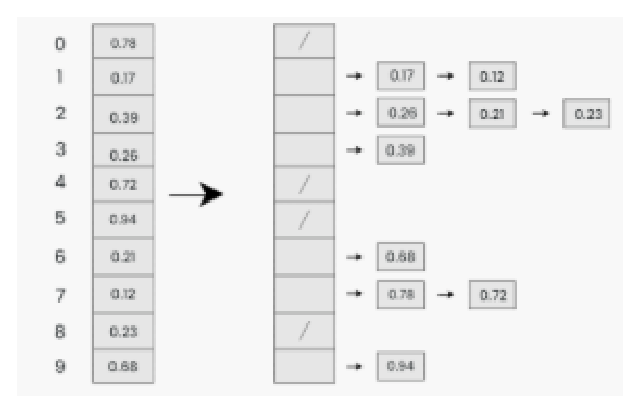
\includegraphics[width=0.8\linewidth]{bucket2.eps}
    \caption{適当に作成されたバケットに要素を入れる。}
  \end{figure}
  \item 各バケット内の要素をソートする(挿入ソートやバブルソートなど、単純なソートでOK)。
  \begin{figure}[H]
    \centering
    \includegraphics[width=0.5\linewidth]{bucket3.eps}
    \caption{各バケットの内容をソートする}
  \end{figure}
  \newpage
  \item すべてのバケットを順番に結合して、最終的なソート済み配列を作る。
  \begin{figure}[H]
    \centering
    \includegraphics[width=0.8\linewidth]{bucket4.eps}
    \caption{バケットを順番に結合}
  \end{figure}
\end{enumerate}
バケットソートの計算量はデータの状況によって定義します.
\begin{description}
  \item[最良] 各バケットには要素の数が同じの場合。
  \begin{equation}
    \centering
    O(n+k)
  \end{equation} 
  \item[平均] 各バケットには要素の数が大分同じの場合。
  \begin{equation}
    \centering
    O(n+k)
  \end{equation}
  \item[最悪] 複数のバケットの間、前要素は同じバケットに入れてしまう状態。
  \begin{equation}
    \centering
    O(n^2)
  \end{equation}
\end{description}
\subsection{カウントソート}
バケットソートと似たように、このソート方法でもバケットみたいの配列を作成する。配列に最高数値を探し、その値を配列の長さとして配列を作成します。データ配列を通過し、その値を前に作成された配列
\section{実験結果}
\end{document}